\documentclass[t,8pt]{beamer}
\usepackage[T1]{fontenc}
\usepackage[english]{babel}
\usepackage[utf8]{inputenc}

% tikz drawing
% ===================================
\usepackage{tikz} % package for creating figures
\usetikzlibrary{calc} % tikz library for calculating
\usetikzlibrary{decorations.pathreplacing}

\usepackage{pgfplots}

\usepackage[framemethod=tikz]{mdframed} % frames

% graphics
% ===================================
\usepackage{graphicx} % importing graphics
\usepackage{transparent} % transparent images

\usepackage{pifont} % symbols

% tables
% ===================================
\usepackage{tabularx}
\usepackage{multirow} % two coloum typesetting

% boxes
% ===================================
\usepackage{tcolorbox} % colourful boxes
\tcbuselibrary{listings}
\tcbuselibrary{breakable}
\tcbuselibrary{skins}

% math
% ===================================
\usepackage[mathcal]{euscript} % math symbols

% algorithms
% ===================================
\usepackage{algorithm} % algorithms
\usepackage{algpseudocode} % style for algorithms

% references
% ===================================
\usepackage{cleveref}

% two column type setting
% ===================================
\usepackage{multicol}

% listings
% ===================================
\usepackage{listings}

% misc
% ===================================
\usepackage{hyperref}
% Variable definitions
% =============================================
% Variable deeptoc (deep or flat table of contents)
\newcommand{\dwDeepToc}[1]{
	\newboolean{deeptoc}
	\setboolean{deeptoc}{#1}
}

% Variable loflot (print list of figures/tables)
\newcommand{\dwLofLot}[1]{
	\newboolean{loflot}
	\setboolean{loflot}{#1}
}

% Adjust font
% =============================================
\renewcommand*\familydefault{\sfdefault}

% Framed Floatings
% =============================================
% Define myBox
\newmdenv[
	innerlinewidth=0.1mm,
	roundcorner=4pt,
	linecolor=black,
	innerleftmargin=6pt,
	innerrightmargin=6pt,
	innertopmargin=6pt,
	innerbottommargin=6pt
]{mybox} 

% Framed figure
\newcommand{\dwFramedFigure}[3]{
	\begin{figure}
		\begin{mybox}
			\centering
     			#1
  		\end{mybox}
  		\vspace{-4.5mm}
  		\caption{#2}
  		\label{#3}    
	\end{figure}
	\vspace{-3mm}
}

% Align two figures next to each other
\newcommand{\dwDoubleFloating}[5]{
%	\noindent\makebox[\textwidth][c]{%
		\begin{minipage}{#2\textwidth}
			#1
		\end{minipage}
		\ifx&#3&\hfill\else\hspace*{#3}\fi
		\begin{minipage}{#5\textwidth}
			#4
		\end{minipage}
%	}
}

% Framed table
\newcommand{\dwTable}[4]{
	\begin{table}
		\tcbox[
			center title,
			colframe=black,
			colback=white,
			boxrule=0.8pt,
			left=-1.2mm,right=-2.3mm,
			top=0mm,bottom=0mm,
			boxsep=0mm,toptitle=0.0mm,
			bottomtitle=0.5mm
		]{
			%\arrayrulecolor{black}
			\renewcommand{\arraystretch}{#4}
			#1
		}
		\vspace{-2.5mm}
		\caption{#2}
		\label{#3}
	\end{table}
}

% Framed listing
% Einstellungen für R-Listings
\lstdefinestyle{r}{
	language={R},
	otherkeywords={},
	morekeywords={eol, TRUE, FALSE},
	deletekeywords={
		<-, _, file, path, ts, pos, !, /, *, =, !=, &&, col,
		data, eval, start, sum, D, mean, find, distance, q, model, predict, gamma, seq
	}
}
\renewcommand*\thelstnumber{\makebox[3em][r]{\ifnum\value{lstnumber}<10 0\fi\the\value{lstnumber}}}
\newtcblisting{dwListing}[1][]{
	enhanced,
	listing only,
	colback=black!5,
	colframe=black!70,
	overlay={
		\begin{tcbclipinterior}
			\fill[black!25] (frame.south west) rectangle ([xshift=5.1mm]frame.north west);
		\end{tcbclipinterior}
	},
	listing remove caption=false,
	left=-1mm,right=-1mm,
	listing options={
		style=tcblatex,
		style=r,
		keywordstyle=\bfseries\color{violet},
		commentstyle=\itshape\color{green!50!black},
		stringstyle=\color{blue},
		numbers=left,
		xleftmargin=7mm,
		tabsize=4,
	},
  	#1
}

% Sections and subsections
% =============================================
% Section command
\newcommand{\dwSection}[1]{
	\ifthenelse{\boolean{deeptoc}}{
		\section{#1}
	}{
		\section{#1}
		\subsection*{#1}
	}
}

% Subsection command
\newcommand{\dwSubsection}[1]{\subsection{#1}}

% Header
% =============================================
% Green header
\newcommand{\dwHeader}[1]{%
\begin{tcolorbox}[
	boxrule=0.2mm,
	boxsep=-1mm,
	lowerbox=ignored,
	colback=green,
	colframe=black,
	hbox
]
	\textbf{#1}
\end{tcolorbox}
}

% Centered version of green header
\newcommand{\dwCenteredHeader}[1]{%
\begin{center}
	\header{#1}
\end{center}
}

% Alert box
% =============================================
\newcommand{\dwAlertBox}[1]{
\hspace*{0.25mm}
\begin{minipage}[c]{0.05\textwidth}
	
\begin{tikzpicture}
		\draw[thick,fill=lightgray] (4.2,0) -- (4.5,0.5) -- (4.8,0) -- (4.2,0) -- cycle;
		\fill[] (4.45,0.17) rectangle (4.55,0.37);
		\fill[black] (4.55,0.08) arc (0:360:0.05);
	\end{tikzpicture}
\end{minipage}
\hfill
\begin{minipage}[c]{0.92\textwidth}
	\begin{mybox}
		\textcolor{red}{\textbf{#1}}
	\end{mybox}
\end{minipage}
}

% Custom itemize environment
% =============================================
\newenvironment{dwItemize}{
\begin{itemize}
\setlength\itemsep{0.8em}
}{
\end{itemize}
}

\newenvironment{dwInnerItemize}{
\vspace{1mm}
\begin{itemize}
\setlength\itemsep{0.8em}
}{
\end{itemize}
}

% Frames
% =============================================
\newenvironment{dwHeaderFrame}[1]{
\subsubsection{#1}
\begin{frame}{#1}
}{
\end{frame}
}

\newenvironment{dwHeaderFrameFragile}[1]{
\subsubsection{#1}
\begin{frame}[fragile,environment=dwHeaderFrameFragile]{#1}
}{
\end{frame}
}

\newenvironment{dwFrame}{
\begin{frame}
}{
\end{frame}
}

\newenvironment{dwFrameFragile}{
\begin{frame}[fragile,environment=dwFrameFragile]
}{
\end{frame}
}

% Print title frame
% =============================================
\newcommand{\dwPrintTitle}[2]{{
	\usebackgroundtemplate{
		\begin{tikzpicture}[]
			\path (0,0) -- (0,10);
			\draw[double,ultra thick, blue!80] (0,7.75) -- (9.5,7.75) -- (9.5,0);
			\draw[double,ultra thick, blue!80] (3,10) -- (3,3) -- (14,3);
			\node at (6,8.5) {};

			\node at (6.25,5.375) {\includegraphics[width=6.2cm,height=4.5cm]{#1}};
			\node[blue!60] at (6.25,2.25) {\textbf{\insertauthor}};
			\node[blue!60] at (6.25,1.75) {\textbf{\insertdate}};
			\node[blue!60] at (6.25,1.25) {\textbf{\insertinstitute}};
			
			\node at (1.5,9) {\includegraphics[width=2.5cm,height=1.5cm]{#2}};
			\node at (7.9,9) {
				\begin{tcolorbox}[
					skin=enhanced,
      					boxrule=0.6mm,
					boxsep=0mm,
					lowerbox=ignored,
					colback=orange!60!red,
					colframe=black,
					borderline={0.5pt}{3pt}{black},
					borderline={1pt}{2pt}{red},
					width=0.75\textwidth
				]
					\centering
					\Large\textbf\inserttitle\par
				\end{tcolorbox}
			};
		\end{tikzpicture}
	}
	\begin{frame}[plain]
	\end{frame}
}}

% Print table of contents
% =============================================
\newcommand{\dwPrintToc}[1]{
	{
		\makeatletter
   		 	\setbeamertemplate{headline}[default]
   			\def\beamer@entrycode{\vspace*{-\headheight}}
		\makeatother

		\begin{frame}[allowframebreaks]
			\begin{tcolorbox}[
				boxrule=0.4mm,
				boxsep=-0.5mm,
				lowerbox=ignored,
				%colback=yellow!60!orange,
				colframe=black
			]
				\centering
				\huge\textbf{Agenda}%
			\end{tcolorbox}
			\vspace{2mm}

			\renewcommand{\baselinestretch}{#1}\normalsize
				\tableofcontents
				
				\ifthenelse{\boolean{loflot}}{
					\framebreak
					\begin{tcolorbox}[
						boxrule=0.4mm,
						boxsep=-0.5mm,
						lowerbox=ignored,
						%colback=yellow!60!orange,
						colframe=black
					]
						\centering
						\huge\textbf{Figures and Tables}%
					\end{tcolorbox}
					\vspace{2mm}
					
					\large\textbf{List of Figures}\normalsize \\
					\vspace*{1mm}
					\listoffigures
					\vspace*{4mm}
					\large\textbf{List of Tables}\normalsize \\
					\vspace*{1mm}
					\listoftables
				}{}
			\renewcommand{\baselinestretch}{1.0}\normalsize
		\end{frame}
	}
}

% Print last slide
% =============================================
\newcommand{\dwPrintThanks}[2]{{
\usebackgroundtemplate{
	\transparent{#2}\includegraphics[width=\paperwidth,height=\paperheight]{#1}}
	\begin{frame}[plain]
		\vfill
		\begin{tcolorbox}[
			skin=enhanced,
		      	boxrule=0.6mm,
			boxsep=0mm,
			lowerbox=ignored,
			colback=orange!60!red,
			colframe=black,
			borderline={0.5pt}{3pt}{black},
			borderline={1pt}{2pt}{red}
		]
			\centering
			\Huge\textbf{Thank you very much \\ for your attention!}%
		\end{tcolorbox}
		\vfill
		\textbf{\insertauthor} \\ \vspace{2mm}
		\textbf{\insertdate} \\ \vspace{2mm}
		\textbf{\insertinstitute}
	\end{frame}
}}

% Print separator slide
% =============================================
\newcommand{\dwPrintSep}[4]{
	{
		\makeatletter
   		 	\setbeamertemplate{headline}[default]
   			\def\beamer@entrycode{\vspace*{-\headheight}}
		\makeatother

		\begin{frame}
			\vspace*{-2mm}
			\begin{tcolorbox}[
				boxrule=0.4mm,
				boxsep=-0.5mm,
				lowerbox=ignored,
				colback=yellow!60!orange,
				colframe=black
			]
				\centering
				\huge\textbf{#1}
			\end{tcolorbox}
			\vspace{#3}
			\begin{figure}
				\centering
				\includegraphics[scale=#4]{#2}
			\end{figure}
		\end{frame}
	}
}

% Misc
% =============================================
% double underline
\newcommand{\dwDoubleLine}[1]{
	\underline{\underline{#1}}
}

% icons
\newcommand{\cmark}{\textcolor{green!70!black}{\ding{51}}}
\newcommand{\xmark}{\textcolor{red}{\ding{55}}}

% redefine cref (add a hyperlink)
\let\chyperref\cref % save original command under a new name
\renewcommand{\cref}[1]{\hyperlink{#1}{\textcolor{blue}{$\Rightarrow$ \chyperref{#1}}}}

\let\Chyperref\Cref % save original command under a new name
\renewcommand{\Cref}[1]{\hyperlink{#1}{\textcolor{blue}{$\Rightarrow$ \Chyperref{#1}}}}

% Comment box
\newcommand{\dwCommentBox}[1]{
	\textbf{Comments:}

	\vspace*{2mm}
	\TextField[multiline=true, width=\linewidth,height=#1]{}
}

% title graphic
%\mode
%<all>
%{
%\renewcommand\titlegraphic[2][]{%
%	\edef\inserttitlegraphic{%
%      	\ifx\relax#2\relax\else
%	      		\noexpand\includegraphics[#1]{#2}%
%      	\fi}%
%  	}%
%  	\titlegraphic{}
%}

% Select theme
\usetheme{mystyle}

% Credentials
\title[Musterthema]{Optimierung industrieller Prozesse}
\author{Gedeon, Fabian, Alex, Philip, Daniel}
\date{12.04.2017}
\institute{DHBW Mannheim}

% Number of levels in toc
\dwDeepToc{false}

% List of figures/tables
\dwLofLot{false}

\begin{document}

\dwPrintTitle{images/evolution}{images/logo_dhbw}
\dwPrintToc{1.2}

\dwSection{Betrachtete Algorithmen}

% ================================================================
\begin{dwHeaderFrame}{Genetischer Algorithmus}
	\begin{dwItemize}
		\item Funktionsweise ist der Natur entlehnt.
		\item Initialisierung einer Population.
		\item Bewertung der Individuen mithilfe einer Fitnessfunktion.
		\item \textbf{Operationen:}

		\begin{dwInnerItemize}
			\item Selektion (der Eltern)
			\item Crossover
			\item Mutation
			\item Ersetzung
		\end{dwInnerItemize}

		\item \textbf{Parameter:}

		\begin{dwInnerItemize}
			\item Popualtionsgröße \& Generationsanzahl
			\item Mutationsrate 
			\item Crossoverrate  
		\end{dwInnerItemize}

	\end{dwItemize}
\end{dwHeaderFrame}

% ================================================================

\begin{dwFrame}
	\dwHeader{Funktionsweise des Algorithmus}

	\dwFramedFigure{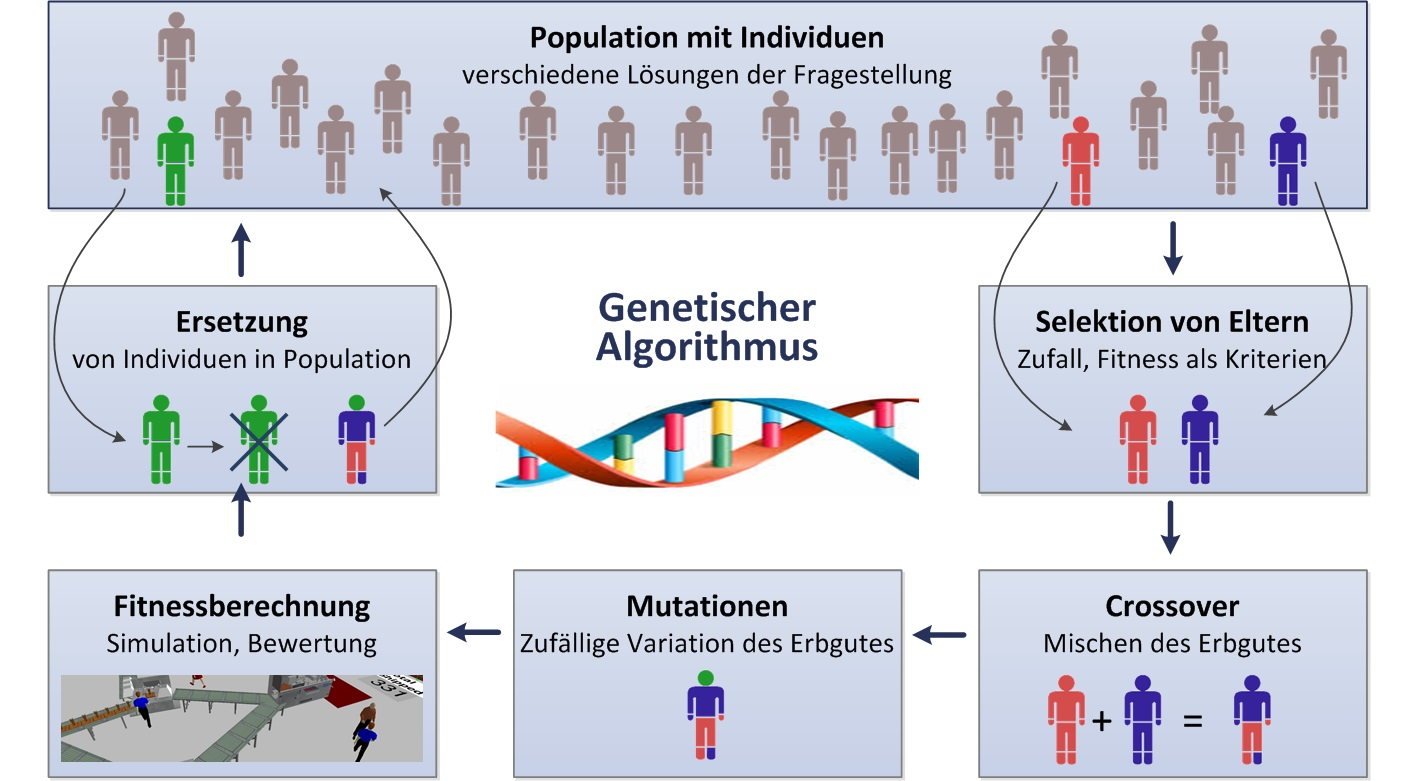
\includegraphics[scale=0.9]{images/genetic_algo}}{Funktionsweise des genetischen Algorithmus}{fig:genetci-algo}
\end{dwFrame}

% ================================================================

\begin{dwFrame}
	\dwHeader{Realisierung}

	\begin{dwItemize}
		\item Crossover-Strategien: 
		
			\begin{dwInnerItemize}
				\item \textbf{Gewichteter Durchschnitt:} Berechnung des gewichteten Durchschnitts (basierend auf der Fitness 								der Eltern) für jedes Gen des Kindes.
				\item \textbf{Singlepoint Crossover:} Kind erhält zwei unterschiedliche Teile des Vektors der Eltern. Trennung 								an einem Punkt. 
				\item \textbf{Multipoint Crossover:} Kind erhält beliebig viele unterschiedliche Teile des Vektors der Eltern. 														Trennung an beliebig vielen Punkten. 
			\end{dwInnerItemize}
		
		\item Mutations-Strategien: 
		
			\begin{dwInnerItemize}
				\item \textbf{Vertauschen zweier Parameter:} Mutationswahrscheinlichkeit für gesamtes Individuum. 										Vertauschen einer festen Anzahl von Genen.
				\item \textbf{Mutation mit fester Anzahl:} Mutationswahrscheinlichkeit für gesamtes Individuum.
							Zufällige Werte für eine feste Anzahl von Genen.
				\item \textbf{Mutation mit variabler Anzahl:} Mutationswahrscheinlichkeit für jedes Gene einzeln.
							Zufällige Werte für eine feste Anzahl von Genen.
				\item \textbf{Gauss Mutation:} Mutationswahrscheinlichkeit für gesamtes Individuum. Addieren eines Gauss-								verteilten Zufallswertes.
			\end{dwInnerItemize}		
		
	\end{dwItemize}
\end{dwFrame}


% ================================================================

\begin{dwFrame}
	\dwHeader{Anpassungen}

	\begin{dwItemize}
		\item Anpassung der Mutationsrate über $e$-Funktion (Optimierung für 5000 Iterationen):\\
			\begin{equation*}
				e^{-x*0.0009-1}
			\end{equation*}
		\item Werte mit \glqq  not feasible\grqq{} werden mit einer Strafe von 1.000.000 für den Fitnesswert versehen. 
		\item Versuch mit fixer Anzahl an Mutationen konsistente Änderungen und Data Space Exploration zu erreichen. 
		\item Truncation Selection mit 25\% der Population 
	\end{dwItemize}
		\vspace{2mm}
	\dwHeader{Parameter}
	\begin{dwItemize}
		\item Populationsgröße: $2^{13}$
		\item Generationsanzahl: 5000
		\item Mutationsrate (variabel): 0.08
		\item Mutationsrate (fix): 0.3 für 4 Individuen
	\end{dwItemize}
		
\end{dwFrame}

% ================================================================
\begin{dwHeaderFrame}{Particle Swarm Algorithmus}
	\begin{dwItemize}
		\item Mehrere Partikel
	\end{dwItemize}
\end{dwHeaderFrame}

% ================================================================
\dwSection{Erkenntnisse}
\begin{dwHeaderFrame}{Genetischer Algorithmus}
	\begin{dwItemize}
		\item Gute Näherung der Testfunktionen von Stiblinski-Tang und Rastrigin.
		\item Schlechte Näherung der Testfunktion von Rosenbrock.
		\item Gute Näherung der unbekannten Funktion
		\item Ergebnisse: \url{https://github.com/DaWe1992/OIP/blob/master/Results.md}
		\item Keine Eignung für alle Optimierungsprobleme
	\end{dwItemize}
\end{dwHeaderFrame}
% ================================================================

\begin{dwHeaderFrame}{Particle Swarm Algorithmus}
	\begin{dwItemize}
		\item Gute Näherung der Testfunktionen von Rosenbrock
		\item Gute Näherung der unbekannten Funktion
	\end{dwItemize}
\end{dwHeaderFrame}
% ================================================================
\dwSection{Kommunikation}
\begin{dwHeaderFrame}{Anbindung an RabbitMQ}
	\begin{dwItemize}
		\item RabbitMQ Client kapselt Funktionalität von Sender und Receiver.
		\item RabbitMQ Client bietet \glqq Send and Wait\grqq{} $\Longrightarrow$ Blockierender Aufruf.
		\item Wiederverwendbarkeit für sämtlich Algorithmen.
	\end{dwItemize}
	\vspace{2mm}
\dwHeader{Technische Limitation}
	\begin{dwItemize}
		\item Maximales Senden von 20k Nachrichten pro Sekunde.
	\end{dwItemize}

	\begin{center}
		
\includegraphics[scale=0.4]{images/rabbitmq}
	\end{center}
	
\end{dwHeaderFrame}


% ================================================================

\end{document}